\chapter{Разработка расчетной сетки и отображение свойств местности на узлы сетки}
\label{chap_mesh}

\section{Расчетная сетка в методе конечных элементов}
\label{sec_fin_elem_mesh}

Для решения уравнения адвекции-диффузии, описанного в разделе \ref{diffusion_model}, в модели \ac{ascro} применяется 
метод конечных элементов. В этом методе область, в которой ищется решение уравнения, разбивается на конечное количество 
подоблостей. Каждая из этих подобластей называется элементами. В каждом элементе выбирается вид аппроксимирующей функции. 
Вне своего элемента аппроксимирующая функция равняется нулю. Значения функций в узлах элементов заранее неизвестны и 
являются решением задачи. Вначале ищутся коэффициенты аппроксимирующих функций из условия равенства соседних функций в 
узлах элементов. После этого, коэффициенты выражаются через значения функций в узлах элементов. Составляется система 
линейных алгебраических уравнений, количество уравнений в которой равно количеству неизвестных значений в узлах, в 
которых ищется решение системы. 

Расчетная сетка в модели \ac{ascro} имеет форму цилиндра и представляет собой участок местности вблизи \ac{aes}. 
Так как расчетная сетка имеет форму цилиндра, её элементы должны быть трехмерными.

Существует четыре основных типа трехмерных элементов: тетраэдры, гексаэдры, призмы и пирамиды (рисунок 
\ref{fig_finite_elements}). Самым распространенным элементом при построении расчетных сеток являются тетраэдры. 

\begin{figure}[ht]
\centering
	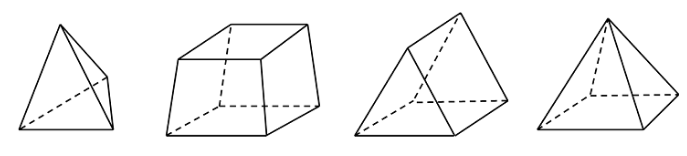
\includegraphics[width=16cm]{finite_elements}
	\captionsetup{justification=centering}
    \caption{Основные типы трехмерных элементов расчетной сетки.}
    \label{fig_finite_elements}
\end{figure}

Тетраэдрический элемент является простейшим элементом и позволяет построить расчетную сетку практически для любого 
трёхмерного тела. В модели \ac{ascro} для решения уравнения адвекции-диффузии методом конечных элементов используется 
расчетная сетка с тетраэдрическими элементами.

\section{Создание расчетной сетки}
\label{sec_mesh_gen}

Построение расчетной сетки для решении уравнения методом конечных элементов является сложной задачей, особенно для 
объекта нетривиальной формы. Как правило, создание расчетных сеток представляет собой трудоемкий и кропотливый процесс. 
В современном мире существует ряд технологий, позволяющих упростить создание расчетной сетки: программа \textit{gmsh}, 
предназначенная для построения трёхмерных расчетных сеток для решения задач методом конечных элементов \cite{gmsh_man}, 
а так же библиотека \textit{pygmsh} для языка программирования Python \cite{pygmsh_doc}, предоставляющая удобный 
интерфейс для работы с программой \textit{gmsh}.

Как было отмечено в разделе \ref{sec_fin_elem_mesh}, расчетная сетка в проекте \ac{ascro} имеет цилиндрическую форму. 
Программный модуль, который отвечает за создание расчетной сетки, должен принимать в качестве входных данных такие 
параметры, как: высота рассматриваемой области в метрах, радиус рассматриваемой области в метрах и шаг между соседними 
узлами расчетной сетки.

Важной задачей является выбор шага между узлами расчетной сетки. Согласно \cite{mke}, точность решения уравнения методом 
конечных элементов во многом зависит от качества разбиения исходной области на конечные элементы и от числа узлов 
конечных элементов. Таким образом, чем гуще расчетная сетка, тем ближе решение, полученное численным методом конечных 
элементов, к аналитическому решению. 

В литературе приводится 2 основных понятия, определяющих радиус рассматриваемой области. Во-первых, это 
санитарно-защитная зона - <<территория (обычно радиусом 3—5 км вокруг промплощадки АЭС), на которой потенциально 
возможно облучение, превышающее предельно допустимое>> \cite{aes_security}. Во-вторых, это зона наблюдения - 
<<территория, на которой возможно обнаружение влияния радиоактивных отходов АЭС и облучение населения может достичь 
предельно допустимых показателей>> \cite{aes_security}. Зона наблюдения может простираться на 25-30 километров от 
\ac{aes}. На санитарно-защитной зоне и зоне наблюдения осуществляется радиационный контроль. В связи с этим, радиус 
рассматриваемой области выбирается исходя из максимального расстояния, на котором осуществляется радиационный контроль, 
то есть на расстоянии 30 километров, соответствующем величине зоны наблюдения.

Так как радиус рассматриваемой области составляет 30 км вокруг источника выброса радиоактивных примесей (вокруг \ac{aes}), 
делать сетку с одинаковым шагом по всей рассматриваемой области не эффективно с точки зрения вычислительных мощностей 
\ac{evm} (\acl{evm}). Более того, расчет распространения радиоактивных примесей планируется проводить в реальном времени, 
что накладывает ограничение на время расчета. 

В связи с поставленными выше ограничениями, было решено сделать различную густоту расчетной сетки при удалении от 
источника радиоактивных выбросов. Расчетная сетка должна быть достаточно детальной вблизи \ac{aes} и по мере удаленности 
от источника радиоактивных выбрасов становиться более разряженной. Следовательно, шаг расчетной сетки должен меняться.

В итоге, в соответствии с поставленными выше требованиями, был разработан программный модуль генерации расчетной сетки. 
Схема разработанного модуля представлена на рисунке \ref{fig_mesh_gen_scheme}. 

\begin{figure}[ht]
	\centering
	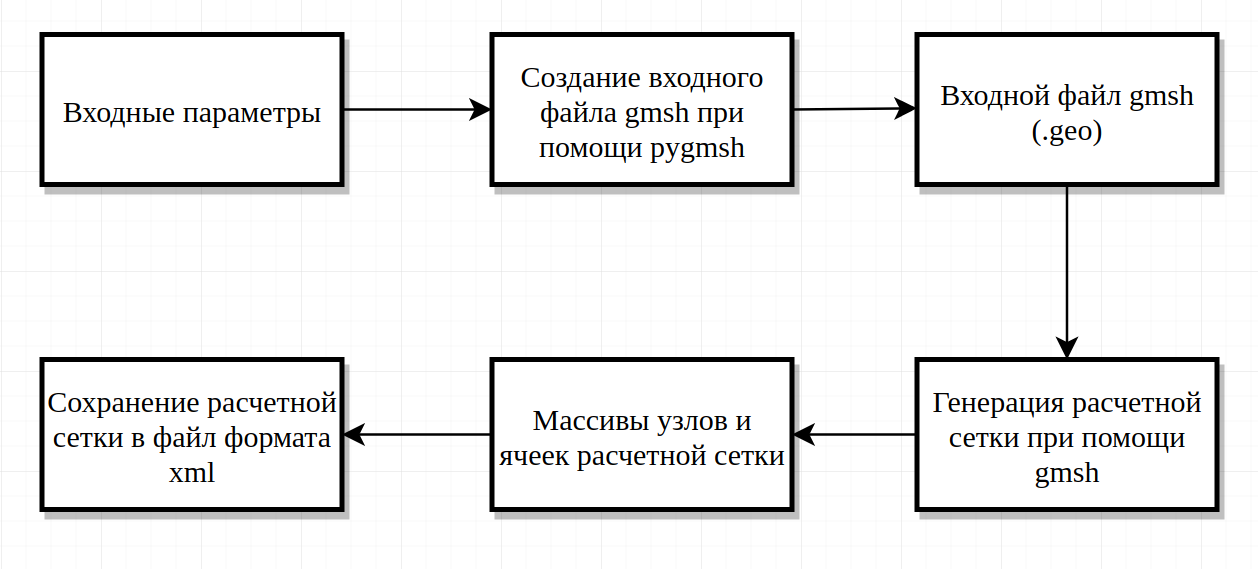
\includegraphics[width=16cm]{mesh_gen_scheme}
	\captionsetup{justification=centering}
    \caption{Схема модуля генерации расчетной сетки.}
    \label{fig_mesh_gen_scheme}
\end{figure}

На вход модуль принимает следующие параметры, необходимые для создания расчетной сетки: высота и радиус рассматриваемой 
области вблизи \ac{aes}; список радиусов, для которых будет задан шаг расчетной сетки; список шагов расчетной сетки для 
каждой области из списка радиусов. Входные параметры задаются в конфигурационном файле проекта.

На втором шаге входные параметры программно считываются при помощи языка программирования Python и на их основе 
происходит процесс создания входного файла для программы \textit{gmsh}. Для создания входного файла используется 
библиотека \textit{pygmsh}, которая позволяет при помощи удобных абстракций задать необходимую геометрию расчетной сетки 
и на основе полученной геометрии сгенерировать файл, содержащий команды на скриптовом языке \textit{gmsh}, в котором 
детально описываются опорные точки и линии создаваемой геометрии. 

Далее, полученный скриптовый файл с расширением \textit{.geo} передается входным параметром программе \textit{gmsh}, 
которая в свою очередь генерирует расчетную сетку. На выходе программа выдает массив, содержащий информацию об узлах и 
ячейках построенной расчетной сетки.

В дальнейшем, для численного решения уравнения адвекции-диффузии методом конечных элементов будет использоваться 
вычислительный пакет \textit{FEniCS}, который требует, чтобы файл расчетной сетки имел формат \textit{xml}. Для этого, 
в модуле генерации расчетной сетки присутствует последний шаг, выполняющий сохранение полученных массивов узлов и ячеек 
сетки в файл формата \textit{xml}.

Пример построенной расчетной сетки при помощи вышеописанного модуля представлен на рисунке \ref{fig_mesh_img}.

\begin{figure}[ht]
	\centering
	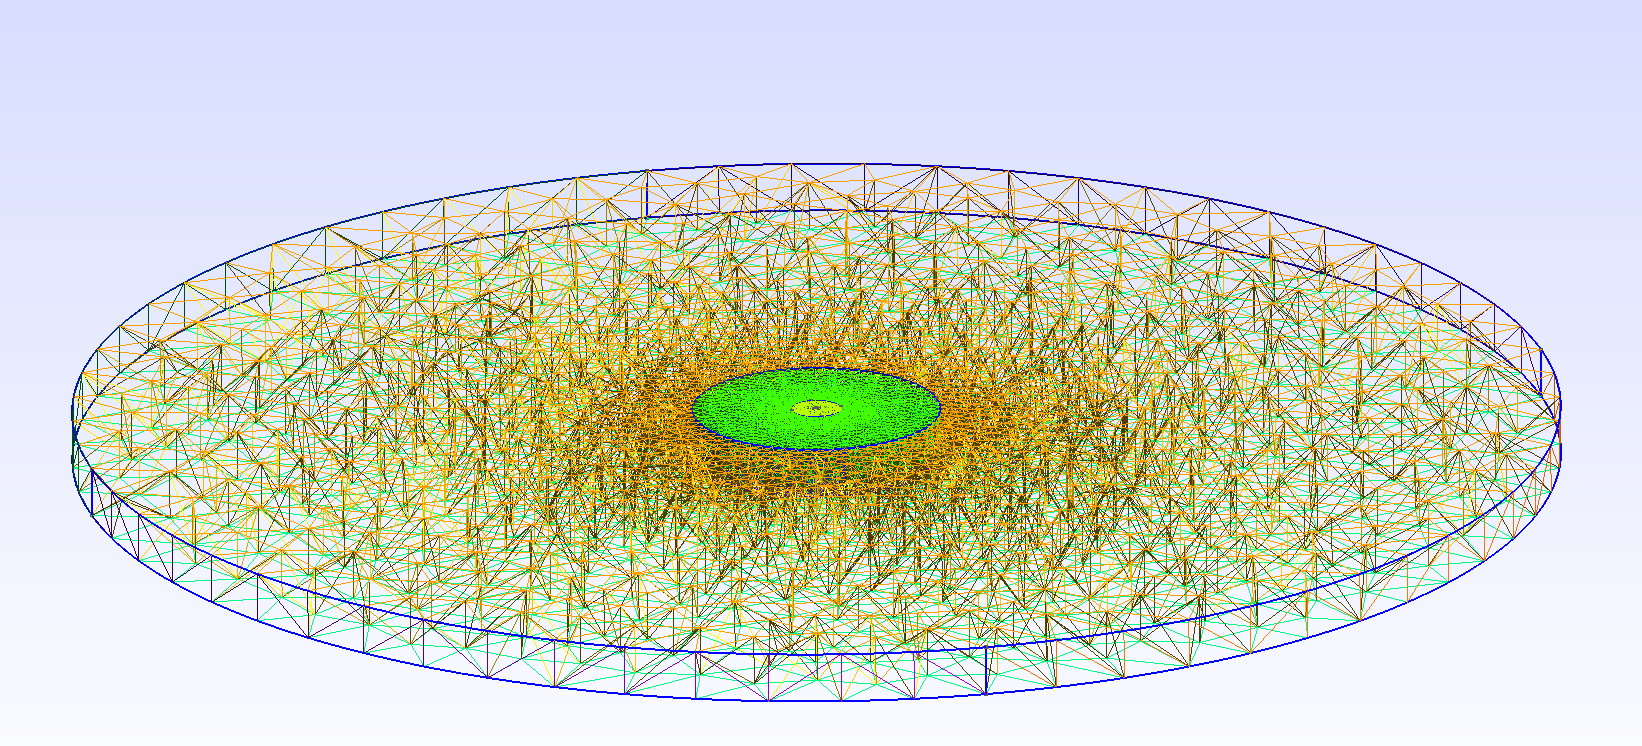
\includegraphics[width=16cm]{mesh}
	\captionsetup{justification=centering}
    \caption{Расчетная сетка, построенная при помощи разработанного модуля.}
    \label{fig_mesh_img}
\end{figure}

\section{Отображение свойств местности на узлы расчетной сетки}

Ранее в главе \ref{chapter_surf_type} был проведен анализ топологической карты местности вблизи \ac{aes} и получено 
соответствие между узлами расчетной сетки и типом подстилающей поверхности. Текущей задачей является разработка модуля, 
отвечающего за отображение свойств, зависящих от типа подстилающей поверхности, на узлы расчетной сетки, необходимое 
для решения уравнения адвекции-диффузии. Такими свойствами являются шероховатость подстилающей поверхности и степенной 
коэффициент для расчета профиля скорости ветра.

Шероховатостью подстилающей поверхности называют неровности подстилающей поверхности, в частности, городские строения, 
растительный покров, снежный покров и прочее, оказывающие значительное влияние на характер распространения воздушного 
потока. Влияние таких неровностей учитывается с помощью изменения параметра шероховатости $z_0$, который является 
табличной величиной и приведен в таблице \ref{table_z0} приложения А для различных типов подстилающей поверхности.

Расчеты перемещения примесей в атмосфере невозможны без учета изменения скорости ветра с высотой. Расчет скорости 
ветра в зависимости от высоты осуществляется c помощью известной зависимости:

\begin{equation}
    \label{eq_wind_distrib}
    u(h) = u_0 (\frac{h}{h_o}) ^ k
\end{equation}

где:
\begin{description}
    \item $u$ - скорость ветра на высоте $h$;
    \item $u_0$ - скорость ветра на высоте флюгера;
    \item $k$ - степенной показатель, зависящий от типа подстилающей поверхности;
    \item $h$ - высота, на которой необходимо рассчитать скорость ветра;
    \item $h_0$ - высота флюгера (в работе принимается равной 10 м).
\end{description}

В работе \cite{roghness_table} приведена эмпирическая зависимость, позволяющая рассчитать степенной показатель $k$ на 
основе шероховатости подстилающей поверхности. Эта зависимость представлена в формуле \ref{eq_k_wind}:

\begin{equation}
    \label{eq_k_wind}
    k = 0,415 + 0,049 \times ln(z_0)
\end{equation}

Кроме того, необходимо учитывать тот факт, что существует пороговая скорость ветра на определенной высоте, выше которой 
скорость ветра не зависит от высоты и является постоянной величиной. Пороговая высота, выше которой профиль скорости 
ветра перестает меняться, зависит от класса устойчивости атмосферы \cite{atmos_doc} и приведена в таблице 
\ref{table_max_wind_height}.

\begin{table}[ht]
    \setlength{\extrarowheight}{1mm}
    \caption{Зависимость пороговой высоты изменения профиля ветра от класса устойчивости атмосферы \cite{atmos_doc}.}
    \label{table_max_wind_height}
    \centering
    \begin{tabular}{|M{0.4\textwidth}|M{0.4\textwidth}|}
    \hline Класс устойчивости атмосферы & Высота $h_{max}$, м \\
    \hline A & 2000 \\
    \hline B & 1500 \\
    \hline C & 1000 \\
    \hline D & 750 \\
    \hline E & 300 \\
    \hline F & 200 \\
    \hline 
    \end{tabular}
\end{table}

Пример профиля скорости ветра при скорости ветра на высоте флюгера равной 5 м/с и классе устойчивости атмосферы A 
в лесной местности представлен на рисунке \ref{fig_wind_distrib}.

\begin{figure}[ht]
    \centering
    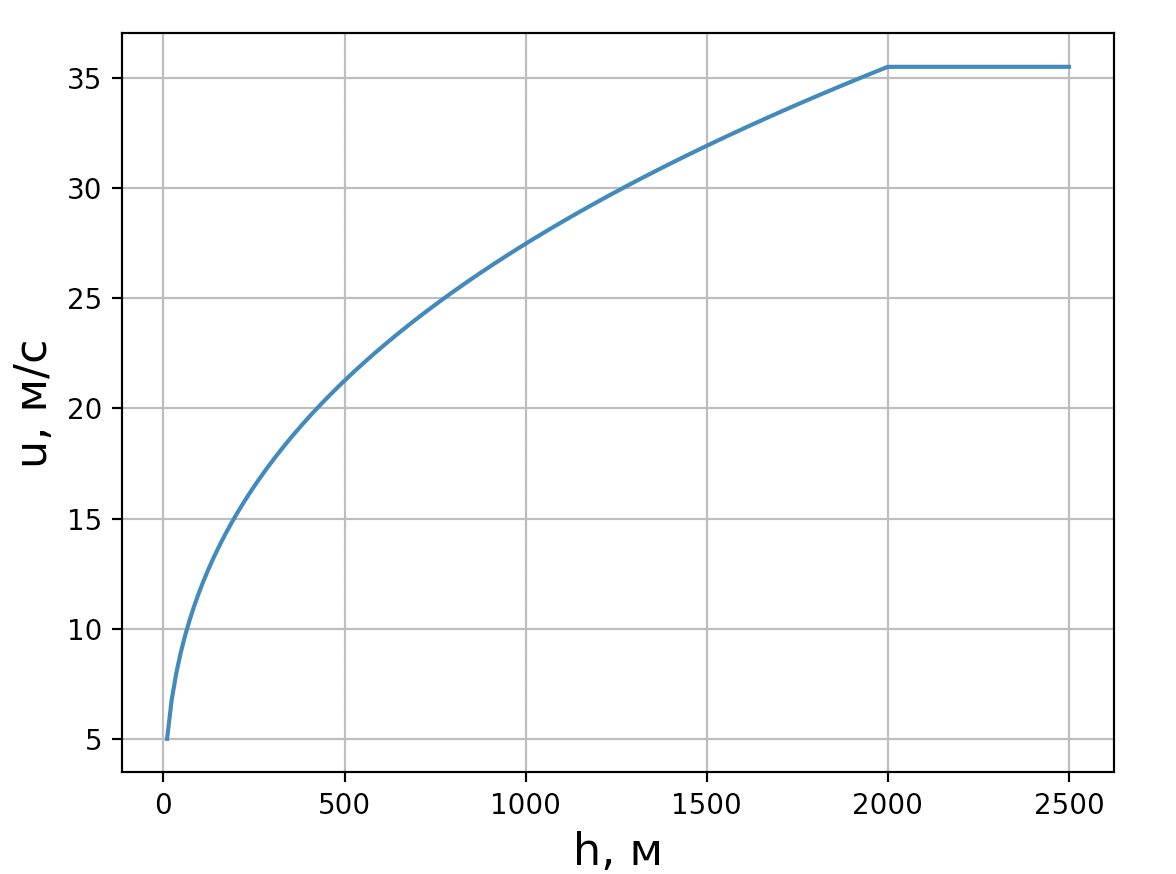
\includegraphics[width=12cm]{wind_distrib}
    \captionsetup{justification=centering}
    \caption{Зависимость скорости ветра от высоты при скорости ветра на высоте флюгера 5 м/с и классе устойчивости 
        атмосферы типа А в лесной местности.}
    \label{fig_wind_distrib}
\end{figure}

На рисунках \ref{fig_z0_distrib}, \ref{fig_wind_x_distrib} представлены примеры работы разработанного модуля отображения 
свойств местности на узлы расчетной сетки. 

На рисунке \ref{fig_z0_distrib} представлен пример отображения шероховатости подстилающей поверхности на узлы расчетной 
сетки, шаг которой одинаков на протяжении всей сетки и составляет 1300 м.

На рисунке \ref{fig_wind_x_distrib} представлен пример отображения продольной составляющей скорости ветра на узлы 
расчетной сетки, шаг которой одинаков на протяжении всей сетки и составляет 1300 м. В данном примере рассматривается 
поперечный срез расчетной сетки на высоте 2000 м при продольной составляющей скорости ветра на высоте флюгера 5 м/с и 
классе устойчивости атмосферы А.

\begin{figure}[ht]
    \centering
    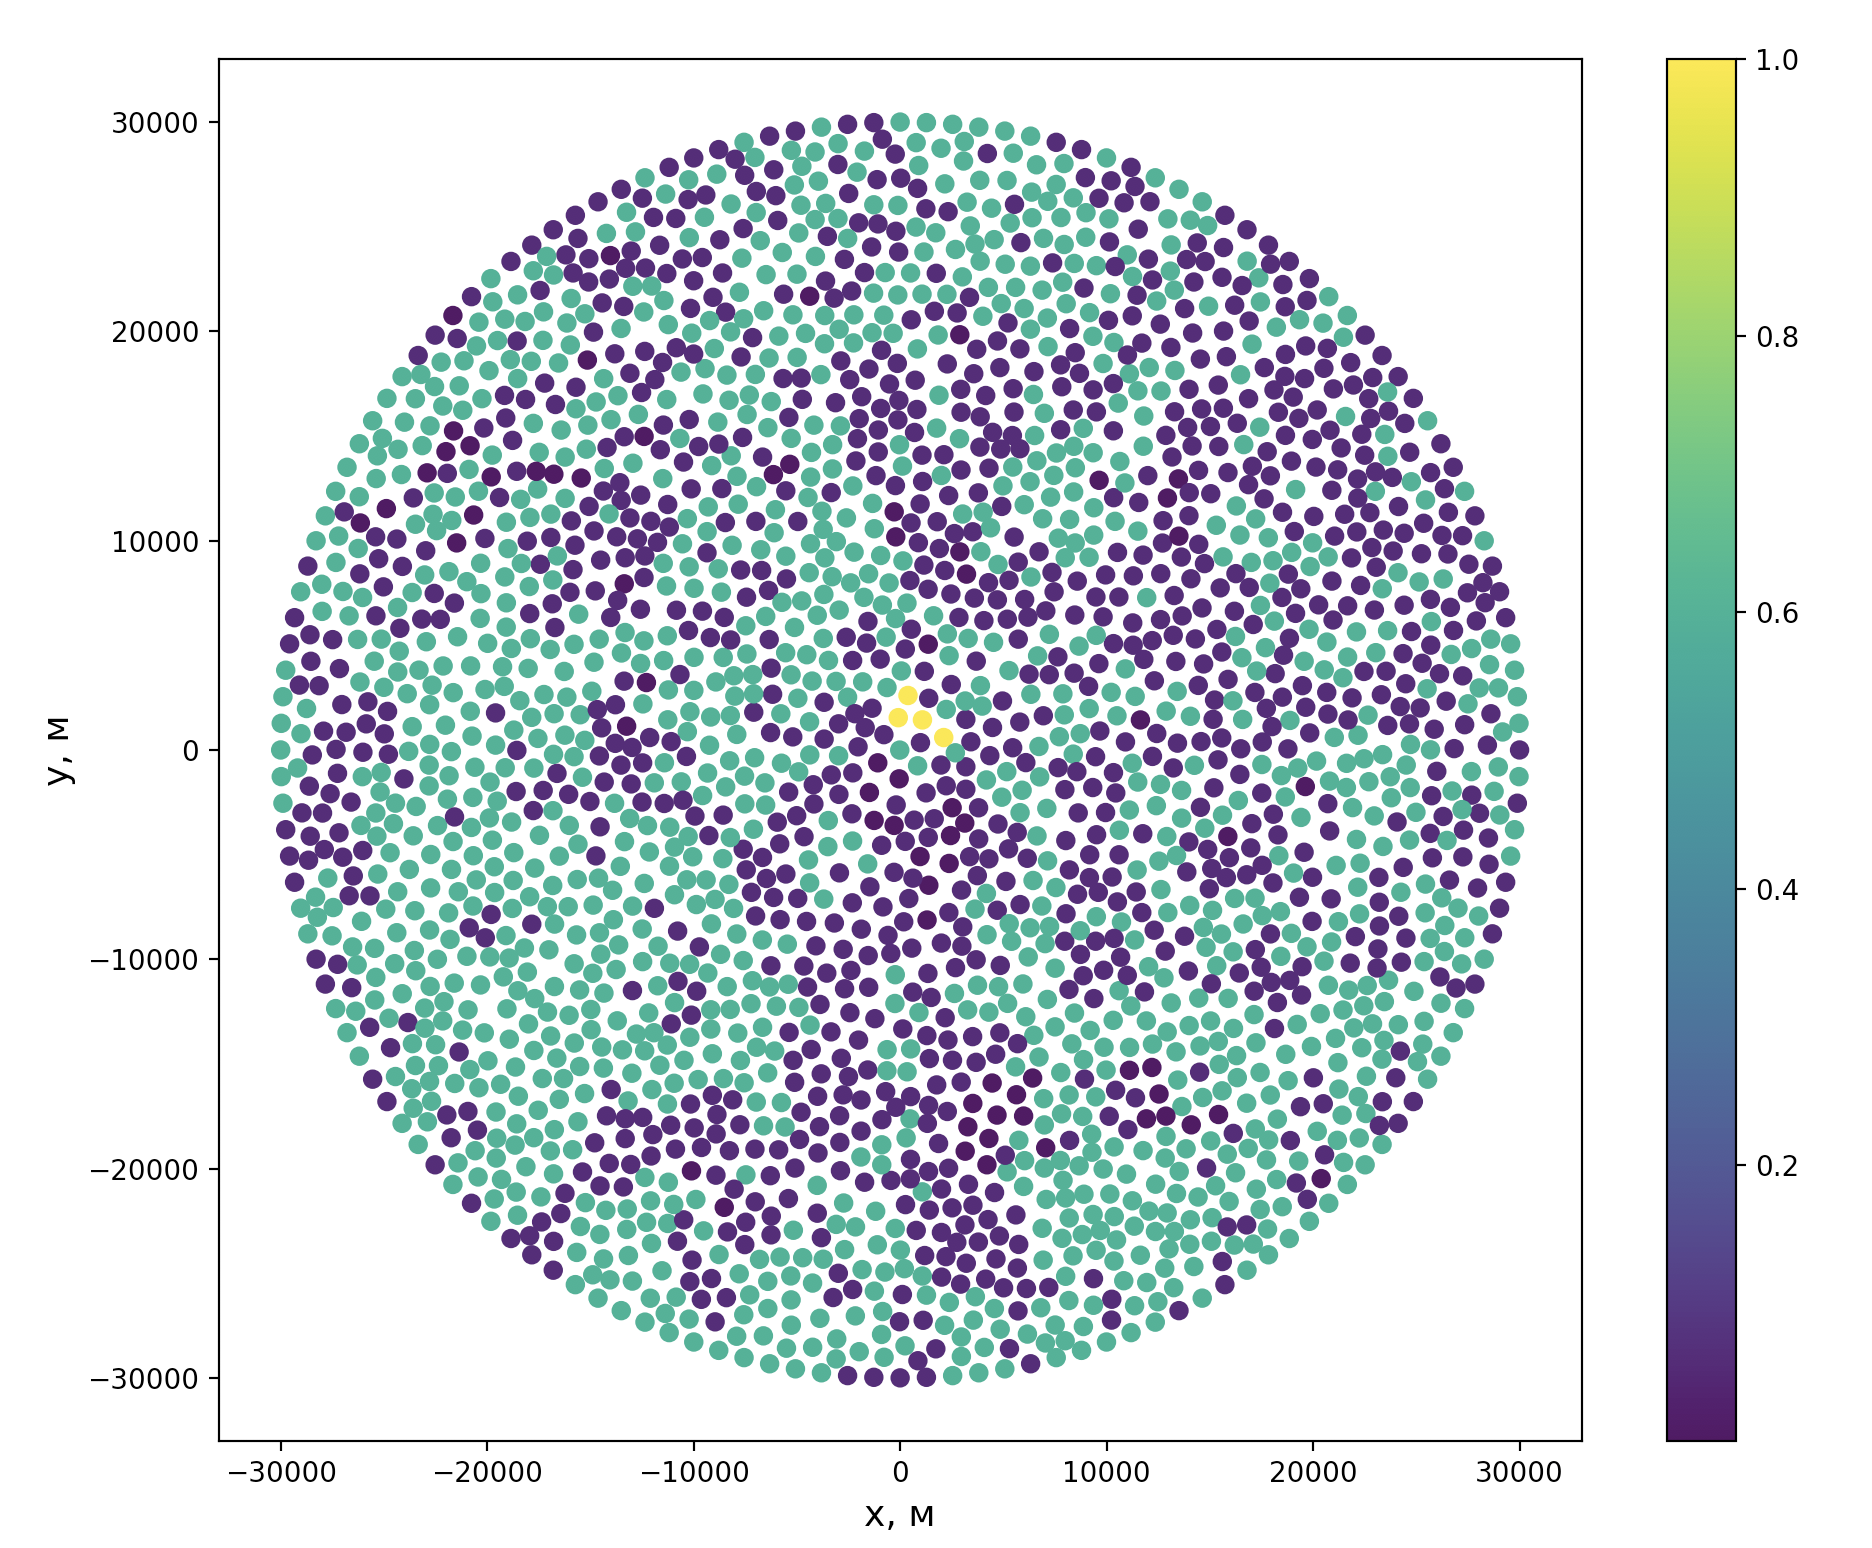
\includegraphics[width=17cm]{z0_distr}
    \captionsetup{justification=centering}
    \caption{Пример распределения шероховатости подстилающей поверхности по узлам расчетной сетки.}
    \label{fig_z0_distrib}
\end{figure}

\begin{figure}[ht]
    \centering
    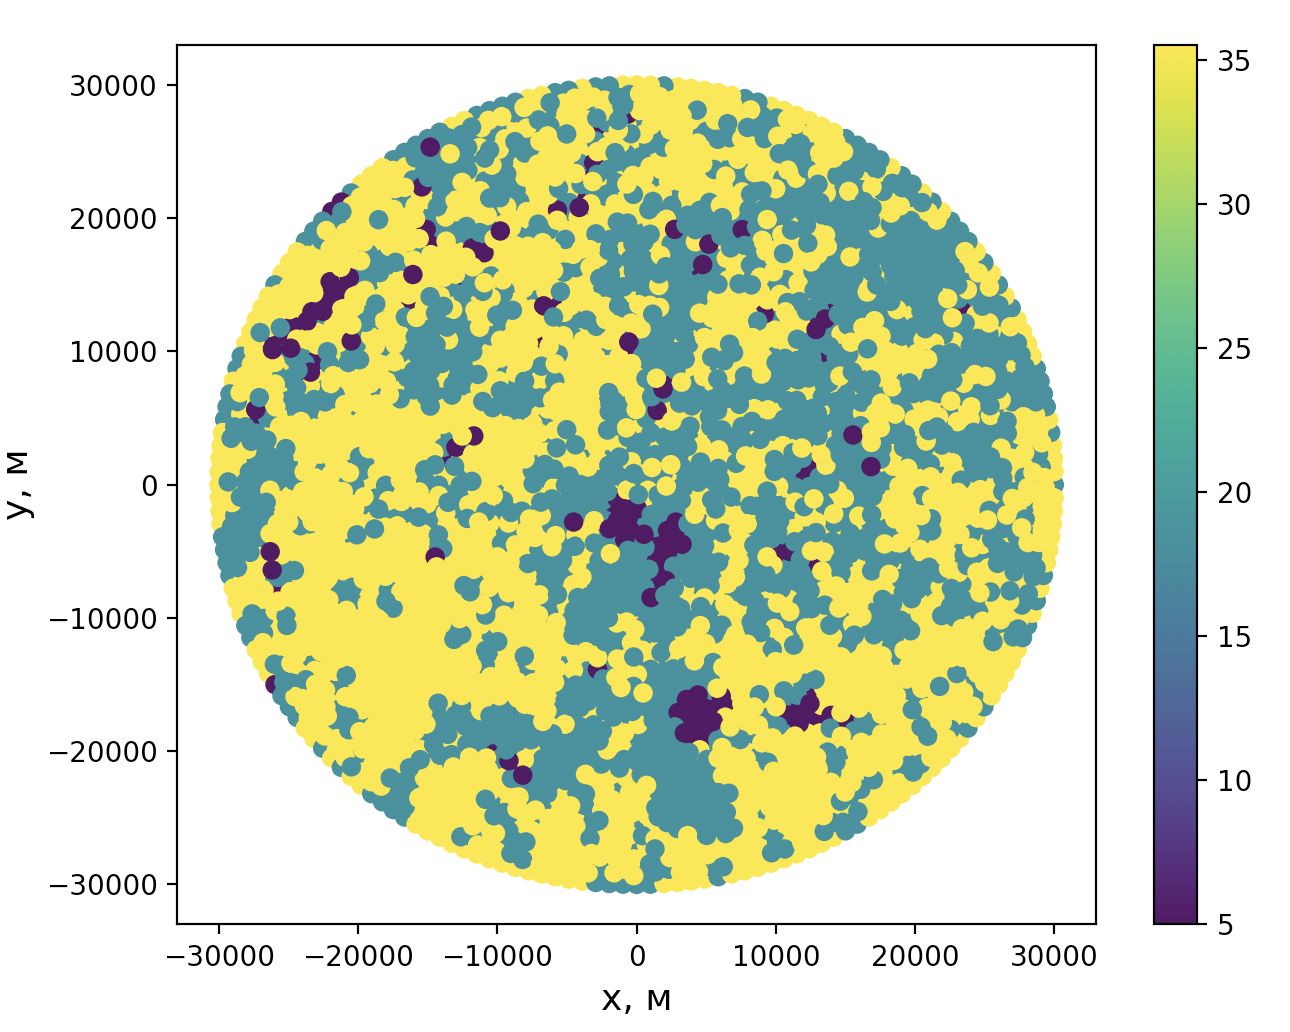
\includegraphics[width=17cm]{wind_x_distr}
    \captionsetup{justification=centering}
    \caption{Пример распределения продольной составляющей скорости ветра по узлам расчетной сетки на высоте 2000 метров 
        при продольной составляющей скорости ветра на высоте флюгера 5 м/с и классе устойчивости атмосферы А.}
    \label{fig_wind_x_distrib}
\end{figure}

В конечном итоге, отображение свойств местности на узлы расчетной сетки сохраняются в файл формата .h5 или .pickle в 
зависимости от параметров, заданных в конфигурационном файле. 

\section{Заключение разработки расчетной сетки и отображения свойств местности на её узлы.}

В данной главе был описан процесс разработки расчетной сетки. Для создания расчетной сетки использовалась программа 
\textit{gmsh}, генерирующая расчетную сетку на основе опорных точек и линий, описанных в скриптовом файле \textit{gmsh}. 
Для упрощения создания скриптового файла \textit{gmsh} использовалась библиотека \textit{pygmsh} для языка 
программирования Python. 

После создания расчетной сетки описывался процесс отображения свойств местности на узлы расчетной сетки. Среди свойств, 
необходимых для решения уравнения адвекции-диффузии и зависящих от типа подстилающей поверхности, выделяются 
шероховатость подстилающей поверхности и степенной коэффициент для расчета профиля скорости ветра. Был разработан 
программный модуль, который на основе данных, полученных в главе \ref{chapter_surf_type}, производит отображение 
вышеописанные свойства на узлы расчетной сетки. Пример работы модуля представлен на рисунках \ref{fig_z0_distrib} и 
\ref{fig_wind_x_distrib}.